\newcounter{nuserstory}

\newcommand{\userstory}[4]{%
    \refstepcounter{nuserstory}
    \subsection{#1}
    \label{userstory:\thenuserstory}
    \hangindent=40pt
    \textbf{\textit{As a}} #2,\\
    \textbf{\textit{I want to}} #3,\\
    \textbf{\textit{so that}} #4.
}


\chapter{Requirement Analysis}
\label{chap:requirement-analysis}

\section{Stakeholder Analysis}
\label{section:stakeholder-analysis}
<TIP: List your stakeholders for your project here/>

Stakeholders are individuals, groups, or entities that
have an interest, concern, or stake in a particular project, decision,
organization, or system. These are individuals or groups who can affect or be
affected by the outcomes of your project.

\section{User Stories}
\label{section:user-stories}

% % user story
% บอก availability of parking lot
% นำทางไปที่ parking นั้นได้
% อยากให้ใส่ destination and see close parking lots that are available or not available
% % parking area owner story
% อยากให้ติดตั้งง่าย
% อยากให้ไม่ต้องใส่จำนวนที่จอดรถเองหรือน้อยที่่สุด
% อยากให้ model ที่ออนไซส์ไม่ต้่องการใช้ computing performance มาก

\userstory{Parking Availability Indicator% 
}{driver on Kasetsart University campus% 
}{see the parking availability indicator% 
}{I don't waste time driving to all parking areas}

\userstory{Navigation to Available Parking% 
}{visiting driver looking for parking% 
}{be guided directly to available parking areas% 
}{I can efficiently reach parking without unnecessary detours}

\userstory{Destination-based Parking Search% 
}{campus visitor% 
}{specify my destination and see nearby parking options with availability status% 
}{I can choose the most convenient parking location for my needs}

\userstory{Existing Infrastructure Utilization% 
}{parking area owner% 
}{implement a parking availability indicator system using existing infrastructure% 
}{I can provide parking information to visitor without significant investment}

\userstory{Lightweight On-Site Resources Requirements% 
}{parking area administrator% 
}{deploy a solution that doesn't require high computing performance on-site% 
}{I can implement the system with existing resources and minimal operating costs}

\section{Use Case Diagram}
\label{section:use-case-diagram}
<TIP: Write a use case diagram for your project here. Refer to an
article “What is a use case diagram?” by Lucidchart for help./>

\section{Use Case Model}
\label{section:use-case-model}
A use case is a detailed description of how a system
interacts with an external entity (such as a user or another system) to
accomplish a specific goal. Use cases provide a high-level view of the
functionality of a system and help in capturing and documenting its
requirements from the perspective of end users.

<TIP: Write use cases for your project here. Make sure to use the
appropriate type of use case for each scenario (brief, casual, and fully-dressed
use case)./>

\section{User Interface Design}
\label{section:user-interface-design}
<TIP: Put the initial design of your application here. You can
showcase a detailed design of a specific page or a sitemap of your application.
See an example below./>

\begin{figure}[h]
    \centering
    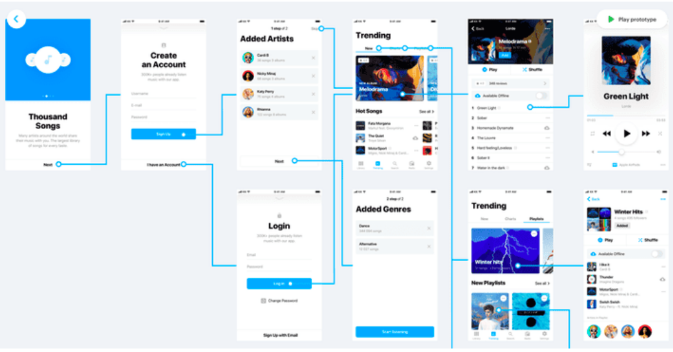
\includegraphics[width=0.8\textwidth]{examples/user-interface-design.png}
    \caption{User Interface Design}
\end{figure}